\chapter{Overall Description}
This section gives a general overview of the factors that affect the product.

\section{Product Perspective}
This section will compare the \gls{ceenc} with other related products and discuss any dependencies.

\subsection{Similar Products}
Before beginning design of the \gls{ceenc}, several alternate \gls{cnc} interfaces were analyzed to understand the current standards and user needs.
While several \gls{cnc} interfaces exist, the \gls{ceenc} has added focus on the usability and lower cost than the alternatives.
\paragraph{MakerBot}
The MakerBot is considered the leader in the current \gls{3d} printer market.
The interface software is MakerBot Desktop, or the older versions were MakerWare.
The MakerBot software allows a user to scan in models and upload files to be printed.
Currently, there is not support for sending files over WiFi, only over USB and Ethernet.
The MakerBot costs around \$2000 depending on the model, although this includes the entire \gls{cnc} machine, not just the driver portion like the \gls{ceenc}.
\paragraph{SmoothieBoard}
SmoothieBoard is an open source driver system with simplistic interfacing software.
It supports Ethernet connections and the system can be accessed through a browser to upload files to the device.
Once a file is uploaded, a command line interface on the device is used to execute files.
The SmoothieBoard costs \$169.97.
\paragraph{EMC2}
EMC2, also known as LinuxCNC, is a freely available \gls{cnc} interface.
It allows for multiple \gls{cnc} configurations, giving flexibility to people who want to build their own \gls{cnc}s.
EMC2 requires a dedicated Linux-based machine and can only operate through a parallel port connector.
\paragraph{OtherMill}
The OtherMill is a new \gls{cnc} controlled by OtherPlan software that costs \$2199.
It allows users to upload a variety of file types, that is converted into G-code interally.
The device offers a command line interface that allows users to send indiviual commands.
The OtherPlan software only supports Mac OS X and the OtherMill must be connected to this computer through USB.

\subsection{Product Dependencies}
The \gls{ceenc} will rely on \gls{tcpip} for communication to a website hosted on the \gls{pi}.
There will be three communication channels in the device, \gls{uart}, \gls{spi}, and gls{i2c}.
The device will be powered from a 12V-36V DC power supply.
The \gls{pi} will be powered from a 5V regulator located on the Control Board.

\section{Product Functions}
The code written for this project is intended to be as modular as possible, avoiding duplication of functionality and increasing testability.
The project relies on free software including the Arch distribution of Linux\cite{archlinux} for the \gls{os} on the \gls{pi}, Apache for web hosting from the \gls{pi}, PHP for creating the back-end services that the website makes calls to, JQuery for creating dynamic web pages, and CuTest, a lightweight unit testing framework for C projects.
As shown in figure~\ref{fig:firmware-hierarchy}, the project contains four software modules: the website control, g-code interpreter, \gls{cnc} driver, and the motor scheduler.
The bootloader on the C2000 is programmed into \gls{rom} and is thus not developed or maintained for this project.
Though not used during normal operation, a set of bash scripts grouped together to create a simple way to set up the \gls{pi} was created to be able to quickly set up the \gls{pi} and get ready for development.

\begin{figure}[!ht]
	\centering
	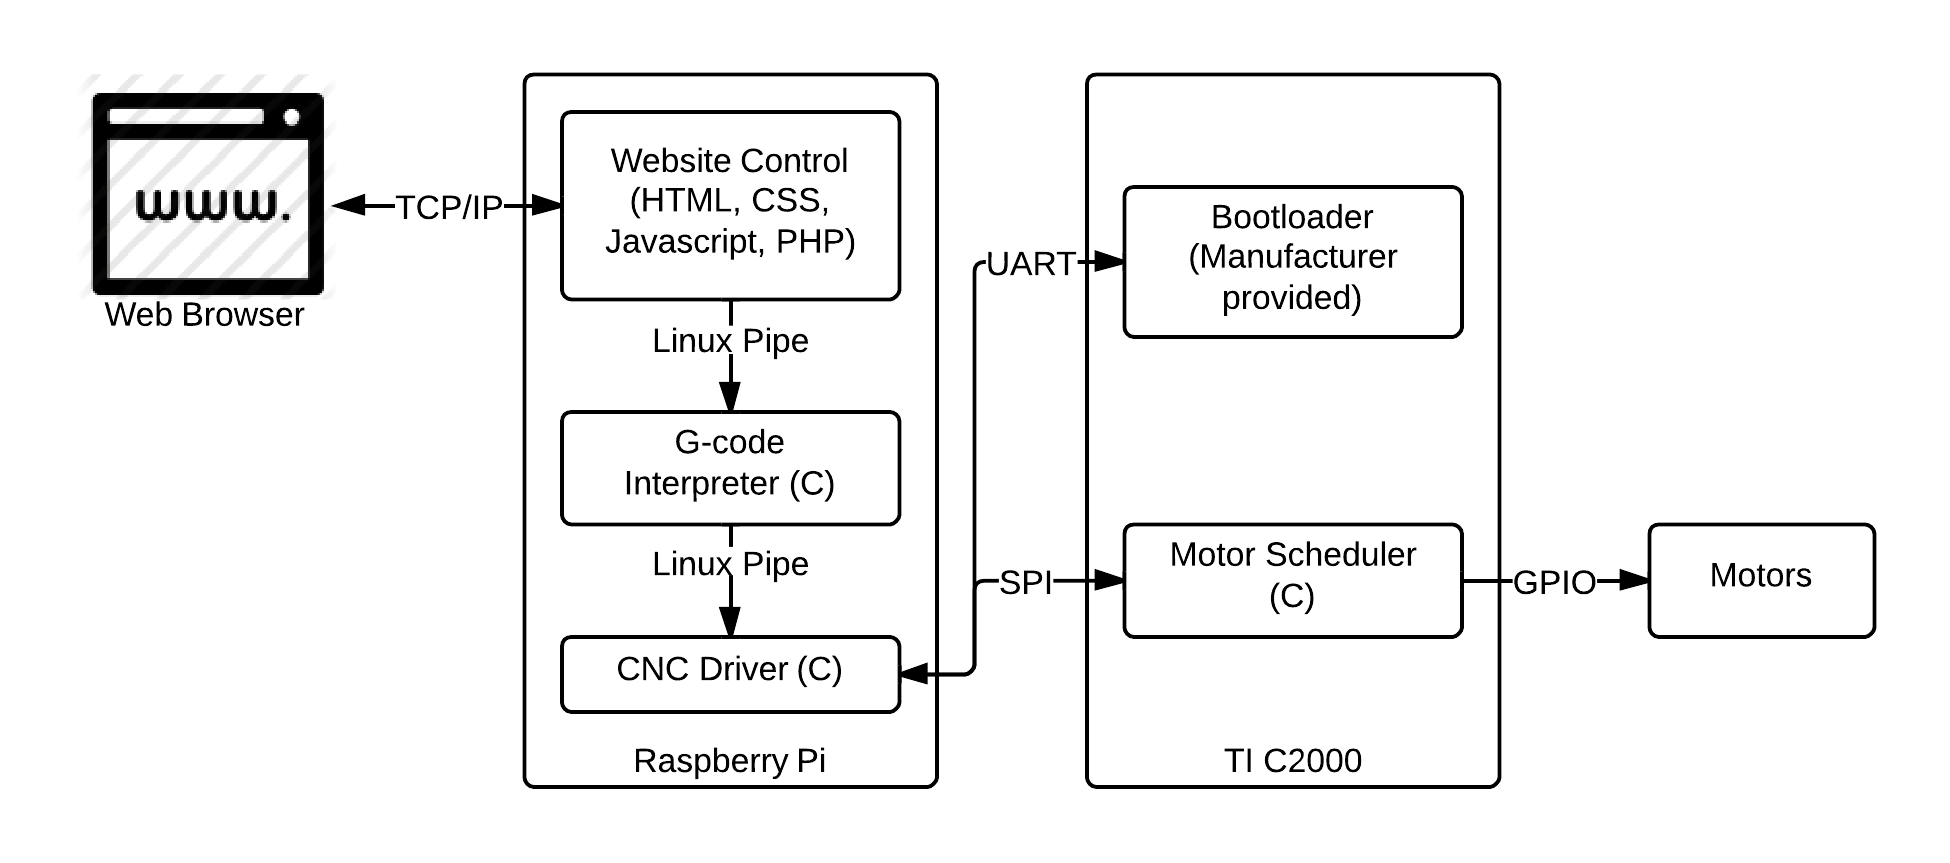
\includegraphics[width=1\textwidth]{firmware-hierarchy.png}
	\caption{Firmware Hierarchy}
	\label{fig:firmware-hierarchy}
\end{figure}

\subsubsection{Website Control}
The website control project is written in HTML, CSS, JavaScript, and PHP and is the main interface between the user and the \gls{cnc}.
The website gives the user the ability to upload, delete, and run g-code files and configure the \gls{cnc}'s characteristics, like gearing ration, maximum speed, and maximum acceleration.

\subsubsection{g-code Interpreter}
The g-code interpreter project is written in C and is responsible for reading g-code line-by-line and interpreting it into instructions for the C2000 to generate the motor pulse trains.
The g-code interpreter listens to a pipe for g-code commands, which may come from a g-code file or directly from the website when the user is homing the machine, then writes to another pipe that is received by the \gls{cnc} driver.
At startup, the g-code interpreter is responsible for driving the state of the C2000, instructing it to home the \gls{cnc}.
The g-code interpreter relies heavily on mathematic formulas created by the software engineer, so many unit tests have been written to ensure proper functionality.

\subsubsection{CNC Driver}
The \gls{cnc} driver project is written in C and is responsible for managing communication channels between the \gls{pi} and C2000 through the \gls{spi} and \gls{uart}.
The g-code interpreter does not write to the \gls{spi} or \gls{uart} directly because these actions require root privileges, so this project was created to allow a single, small program to run as root, while the larger, more frequently changing programs are run by regular users.
The \gls{cnc} driver listens to a pipe for commands to send to the C2000 and forwards them through \gls{spi}, verifying that it is received based on the echo back from the C2000.
The \gls{cnc} driver also looks for a special command that indicates that the next bytes will be \gls{ti} hex data and the program should reset the C2000 and bootload the device with new code.

\subsubsection{Motor Scheduler}
The motor scheduler project is written in C and is responsible for listening for commands from the \gls{pi} and generating the pulse trains to the motors.
The project is based off an algorithm that requires no floating point operations on the C2000 for generating pulses, saving resources and allowing better real-time performance.
The commands are accepted through \gls{spi} and are acknowledged by echoing back the received data, with the command format specified in a C header file shared between the g-code interpreter and this project.

\section{User Characteristics}
The intended users for the \gls{ceenc} will be hobbyists or students interested in computer numerical control for products such as mills or \gls{3d} printers.
The user will be familiar with web interfaces and have access to a \gls{cnc} machine for the interface.
Technical expertise will vary from those who purchase a \gls{cnc} machine pre-assembled to those who make their own and have an understanding of the mechanics involved.
Design of the product will be simple and targeted to those who have little experience with the mechanics involved in a \gls{cnc}.

\section{Constraints}
The major constraints for this project are computational requirements, interface requirements, peripheral requirements, power requirements, packaging requirements, time, and cost.

\subsection{Computational Requirements}
The main computational requirement for this project is the conversion of G-code commands to motor control functions.
The secondary computational requirement is the count and timing of stepper motor steps.
The \gls{pi} will handle software conversion while the microcontroller will handle the timing and count of the motor steps.
When a G-code design file is uploaded and sent to the \gls{pi}, the \gls{pi} will convert the code into commands that can be sent to the microcontroller over a \gls{spi} bus.
This conversion may occur in non-real-time.
The microcontroller will handle the timing and counting of the motor control functions.
Once the microcontroller receives the motor control commands, it will output appropriate step and direction data to the motor drivers.
The motor control data must execute in real-time to ensure accuracy.
The microcontroller must be capable of outputting a step frequency of at least 10kHz and within 5\% of the target frequency for any frequency in that range.
The microcontroller will also monitor the status of the motor drivers and communicate any faults back to the computer.

\subsection{Interface Requirements}
The microcontroller must have at least 8 outputs for stepper motor control, 4 inputs for stepper motor home, 1 input for the motor driver faults, 1 input for an emergency stop, and 1 PWM output for DC motor control.
Between the computer and microcontroller, an additional 16 outputs must be available for use by the end user as part of the project success criteria.
The additional outputs may be accomplished by using serial to parallel shift registers or an \gls{i2c} port expander.
If shift registers are used, 3 output pins will be required by either the pi or microcontroller for the clock, storage input, and data input.
If an \gls{i2c} port expnader is used, 2 output pins will be required by either the \gls{pi} or the microcontroller for the \gls{i2c} channel.
All digital logic will be 3.3V.
To protect the \gls{pi} and microcontroller, opto-isolators will be used at the input and output of the motor drivers.

\subsection{Peripheral Requirements}
The \gls{pi} will require either Ethernet or Wi-Fi capabilities to connect to a website.
The \gls{pi} must have a one channel \gls{spi} bus to communicate with the microcontroller. 
The microcontroller must have a one channel \gls{spi} bus to communicate with the \gls{pi}.
The microcontroller must have a JTAG port for programming.
The microcontroller may require up to four 16-bit timers for motor step counting.

\subsection{Power Constraints}
The system will accept one DC power supply that can be between 14V and 36V.
The system will draw no more than 10A including the current required for the motors.
A 5V power regulator will be used to supply the computer.
A 3.3V power regulator will be used to supply the microcontroller and ICs.
The 14-36V DC rail will be used to supply the motor drivers. 

\subsection{Packaging Constraints}
The finished project must be professionally packaged.
The footprint of the packaging will likely not be much larger than the footprint of largest PCB which is expected to be approximately 87mm x 56 mm, however this is not a requirement.
The size of the finished project will not impact performance in a considerable manner.

\subsection{Time and Cost Constraints}
Current CNC interfaces require use of a full computer system in combination with a motor driver platform.
These setups can cost upwards of \$500.
This project will combine and simplify these hardware and software requirements for a cost of under \$100.
Since this is a student project, there is 

\section{Assumptions and Dependencies}
This subsection of the SRS should list each of the factors that affect the requirements stated in the SRS.
These factors are not design constraints on the software but are, rather, any changes to them that can affect
the requirements in the SRS. For example, an assumption may be that a speciÞc operating system will be
available on the hardware designated for the software product. If, in fact, the operating system is not available,
the SRS would then have to change accordingly.